\section{Introduction}

\begin{figure}[t]
	\centering
		\begin{minipage}{0.225\textwidth}
			\centering
			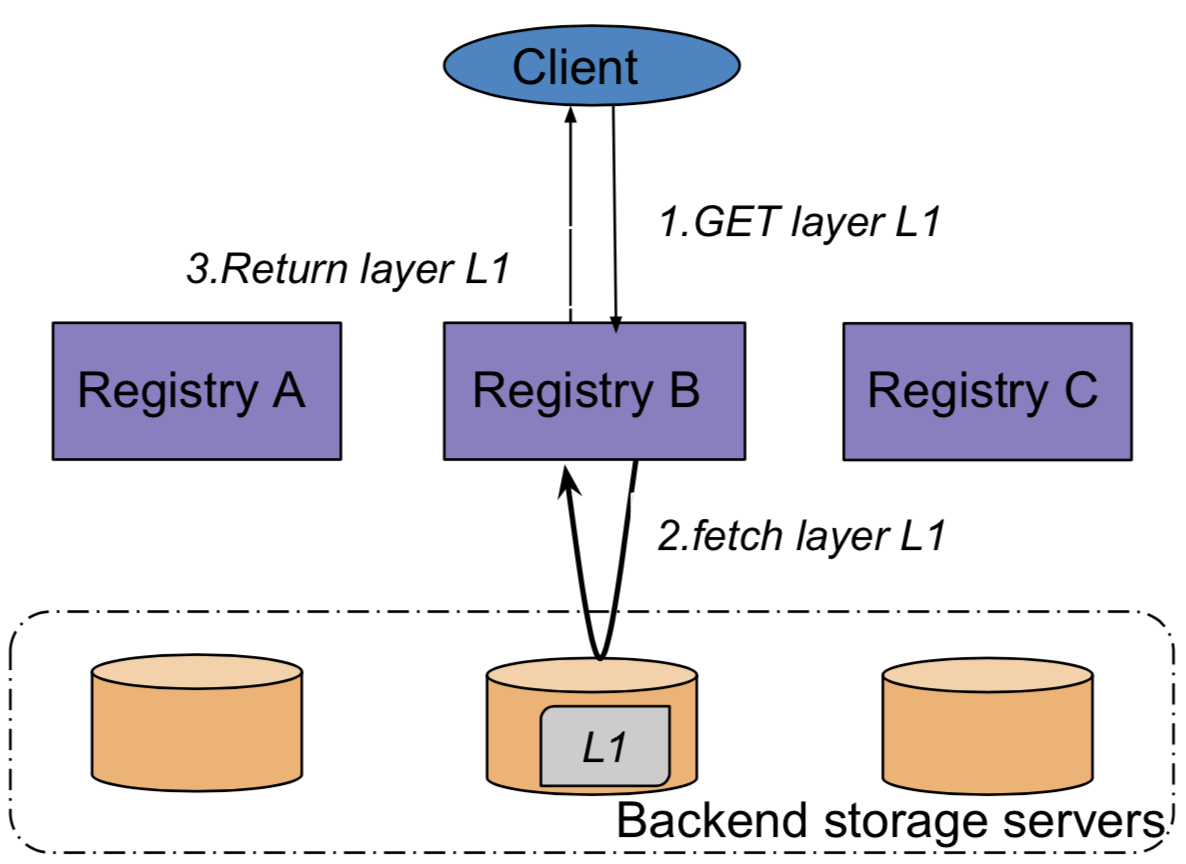
\includegraphics[width=1\textwidth]{graphs/nodedup.png}
			\caption{CDF of layer reference count.}
			\label{fig:ref_count}
		\end{minipage}
	\begin{minipage}{0.225\textwidth}
		\centering
		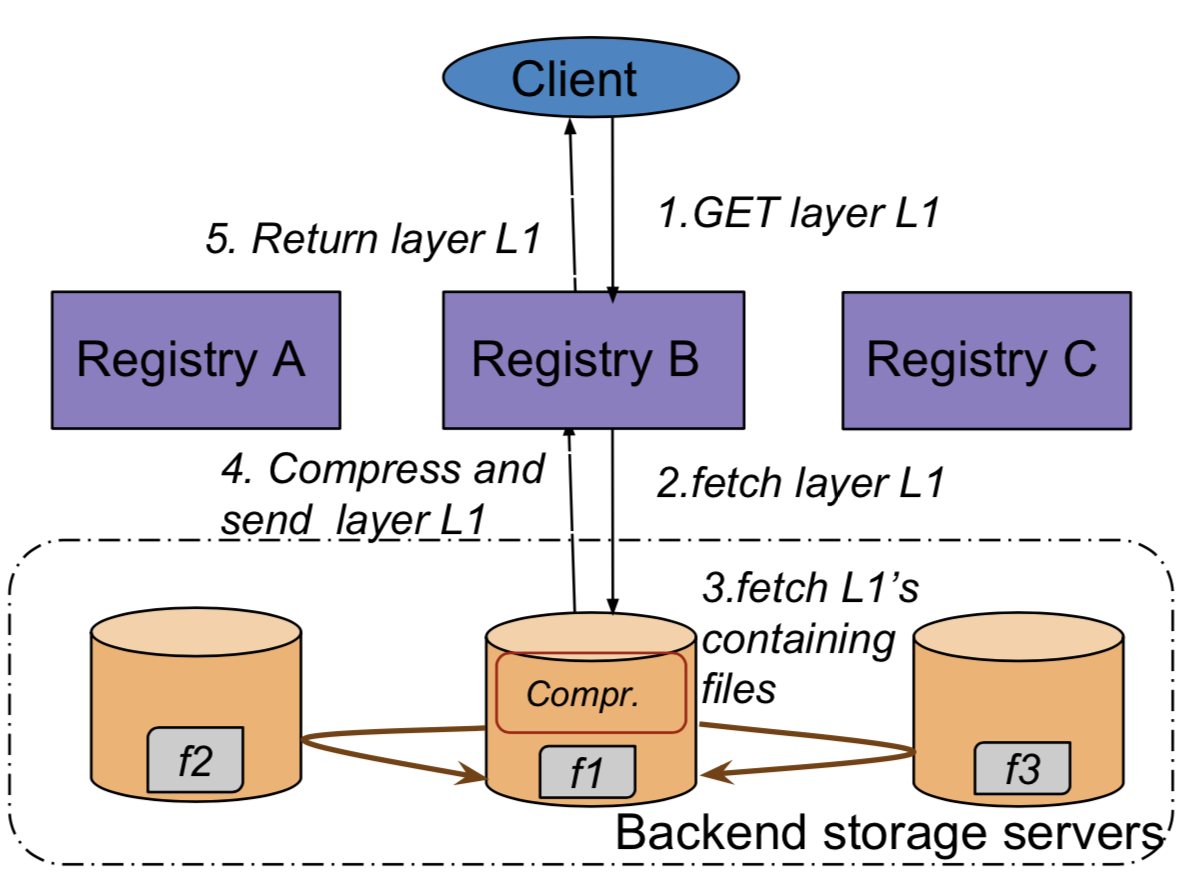
\includegraphics[width=1\textwidth]{graphs/dedup.png}
		\caption{CDF of compress. and uncompress. layer size.}
		\vspace{-3pt}
		\label{fig:nodedup-vs-dedup}
	\end{minipage}
\end{figure}
Due to their tight isolation, low overhead, and efficient packaging of the execution environment, 
Docker containers have become a prominent solution for deploying modern applications.
Containers are created from \emph{images} which are stored in a Docker \emph{registry}. 
An image consists of a list of \emph{layers} which can be shared among images.
Docker registries store a large amount of images and with the increasing popularity of Docker, 
they continue to grow. 
For example, Docker Hub---a popular public registry---stores more than half a million public images.
In this paper, we first analyze over 167\,TB of uncompressed Docker images.
We found only~7\% of the files are unique.
Container images are similar with VM images in the sense that they all serve as OS snapshots. 
Different users might choose similar OS and run similar applications, which incurs a considerable redundancy across different container images.
However, the massive amount of redundant files in the uncompressed image dataset means that 
Docker's existing layer sharing mechanism is not sufficient to eliminate this profound redundancy. 

Deduplication technique is a good solution to remove the redundancy from container image storage system. 
However, current deduplication techniques cannot be directly applied on container image storage system 
because container images are stored as a number of gzip compressed tar files, known as layers. 
Gzip compressed files have very less deduplication ratio. 
We can decompress the layers before applying deduplication on Docker registries
However, restoring layers by assembling files or chunks incurs a considerable additional overhead on pull time
while container service requires high startup speed, which puts a tight constraint on image pull time. 

Therefore, in this paper, 
we propose a low restore latency, adaptive deduplication framework for Docker registries.
%
First, to improve pull performance, we design a user behaviour-oriented cooperative cache
to adaptively host a certain amount of active users' layers for speeding up active users' pull time
and also to selectively store few popular \textit{shared} files for fastening layer restoring process.
% 
Second, to further improve registry performance, we design an elastic deduplication model by combining 
local deduplication and global deduplication methods.
  
The idea of user behavior-oriented cooperative cache is that,
instead of only focusing on layer-level access pattern, we consider user behaviours in cache replacement
because user behaviour is more predictable than layer access pattern and 
users are the ones who issue the layer/manifest pulls/pushes.
Our cache replacement policy is an adaptive heuristic, top-down decision making process driven by user behaviors.
During cache eviction, we first evicts the least recently active users along with the repositories belong to them.
Next, we remove the least recently accessed layer candidates exclusively referenced by these victim repositories to make room for new users' layers. 
For the incoming new users, we prefetch a number of their repositories along with their containing layers based on
their access probabilities.

After an inactive users' layers are evicted from cache, it will be first sent to a local deduplication pool where it will be 
decompressed and the files that have already been stored locally will be removed. 
In this case, restoring these layers won't incur inter-registry file transfer.
If these users stay inactive for a long time,
we will migrate their locally \textit{deduped} layers from local deduplication storage pool to global deduplication pool 
where their containing files that have already been stored globally in the distributed Docker registry system will be removed. 
The \textit{size ratio} between local deduplication pool and global deduplication pool can be elastic based on 
system performance, deduplication ratio, and designers' demand.
Beside, our cache also collaborates with our elastic deduplication pools to store the popular files that are shared among many layers
to speedup restoring performance.

The organization of this paper is as follows:

%%%%%%%%%%%%%%%%%%%%%%%%%%%%%%%%%%%%%%%%%%%%%%%%%%%%%%%%%%%%%%%%%%%%%%%%%%%%%%
%                                                                            %
%                                OLD INTRO                                   %
%                                                                            %
%%%%%%%%%%%%%%%%%%%%%%%%%%%%%%%%%%%%%%%%%%%%%%%%%%%%%%%%%%%%%%%%%%%%%%%%%%%%%%

%\emph{Containers}~\cite{process-containers-linux} have recently gained
%significant traction due to their low overhead, fast deployment, and
%the rise of container management frameworks such as Docker~\cite{docker}.
%%
%Polls suggest that 87\% of enterprises are at various stages of adopting
%containers, and they are expected to constitute a \$2.7 billion
%market by 2020~\cite{container-grow-by2020}.
%
%Docker combines process containerization with efficient and effective packaging
%of complete runtime environments in so called {\em images}.
%%
%Images are composed of shareable and content addressable {\em layers}.
%%
%A layer is a set of files, which are compressed in a single archive.
%%
%Both images and layers are stored in a Docker \emph{registry} and accessed by
%clients as needed.
%%
%Since layers are uniquely identified by a collision-resistant hash of
%their content, no duplicate layers are stored in the registry.
%
%Registries are growing rapidly.
%%
%For example, Docker Hub~\cite{docker-hub}, the most widely used registry,
%stores more than 500,000 public image repositories comprising over 2 million
%layers and it keeps growing.
%%
%Over a period from June to September 2017, we observed a linear growth of the number
%of images in Docker Hub with an average creation rate of 1,241 repositories per day.
%%
%We expect this trend to continue as containers gain more popularity.
%%
%This massive image dataset presents challenges to the registry storage
%infrastructure and so far has remained largely unexplored.
%
%In this paper, we perform the first large-scale redundancy
%analysis of the images and layers stored in Docker Hub.
%%
%We downloaded 47\,TB (167\,TB uncompressed) worth of Docker Hub images,
%%
%which in total contain over 5 billion files.
%%
%Surprisingly, we found that only around 3\% of the files are unique
%while others are redundant copies. This suggests that current layer
%sharing cannot efficiently remove data duplicates.
%%
%We further analyzed the reasons for the high number of redundant files
%and found, for example, that different Docker images often
%contain the same source code from external public repositories
%(e.g., GitHub~\cite{github}).
%%
%%As there are no official images containing this source code, users manually add
%%it to their images, resulting in different layers which cannot be reused.
%
%Given our findings, we propose \sysname, a file-level content addressable storage
%model for the Docker registry.
%%
%\sysname\ unpacks layer tarballs into individual files and deduplicates them.
%%
%When a Docker client requests a layer, \sysname\ dynamically reconstructs the
%layer from its constituent files.
%%
%To assess the feasibility of our design, we conduct a simulation-based
%evaluation of \sysname. 
%%
%The simulation results show that \sysname\ improves the deduplication
%ratio from 1.8$\times$, provided by layer sharing, to 6.9$\times$.
%%provided by file-level deduplication.
%%
%While \sysname\ comes with some overhead 
%%when retrieving layers from the registry
%caused by the need to decompress and reconstruct layers, we found,
%for example, that for
%layers less than 10\,MB (around 60\% of all layers) the overhead of
%retrieving a layer is less than 1\,s.
%%
%For larger layers, we propose several optimizations to reduce overhead.
%\VT{Here we need to add 1-2 *most interesting* performance-related findings.}

%
%The simulation result show that 
%(1)~processing layers in
%parallel can largely improve throughput. For example, 80\% of file-level deduplication time is
%less than 9.09 s per layer and by processing 60 layers in parallel, our one-node
%prototype can process about 3 layers per second.
%
%\LR{That sounds like we actually ran the deduplication and not just simulated it?
%Did we perform more of an \emph{emulation}?}
%
%(2) Fast compression methods can mitigate pull overhead caused by re-compression
%because files are required to be re-compressed as a compressed layer archival file to serve
%the incoming pull requests.
%

%
%We make three major observations:
%
%\begin{compactitemize}
%
%\item Only 10\% of layers are referred to by more than one image, 
%meaning that layer-level content addressability is not enough to
%effectively reduce storage utilization in the registry.
%\DIM{Should we also provide the capacity \%?}
%
%\item A large amount of files are shared across layers and images,
%resulting in only 3\% of unique files.
%\DIM{Should we also provide the capacity \%?}
%
%\item Source code and scripts have a high deduplication ratio
%(\textbf{$31.25\times$} for source codes and \textbf{$50\times$} for scripts),
%which can result in executable and object file duplicates.
%
%\end{compactitemize}


%%%%%%%%%%%%%%%%%%%%%%%%%%%%%%%%%%%%%%%%%%%%%%%%%%%%%%%%%%%%%%%%%%%%%%%%%%%%%%
%                                                                            %
%                                OLD INTRO                                   %
%                                                                            %
%%%%%%%%%%%%%%%%%%%%%%%%%%%%%%%%%%%%%%%%%%%%%%%%%%%%%%%%%%%%%%%%%%%%%%%%%%%%%%

%Finally, we proposed and implemented Docker registry design that performs
%deduplication.
%%
%In our thorough redundant analysis and characterization of the xxxx images,
%with xxxx layers and xxxx files, we investigated the following four research
%questions (RQs):
%
%\begin{compactitemize}
%%
%\item How much redundant data stored in layers, images, and registry? Although
%layer-level address content addressable storage is adopted by Docker, we do not
%know whether  this coarse-grain layer-level content addressable storage (LLCAS)
%can efficiently reduce duplicates, and how much redundant data is stored in
%layer, image, and registry.
%%
%\item What are the redundant files and why there are so many redundant files?
%We aim to identify what are the redundant files that users mostly replicate.
%%
%Such information will provide Docker designer knowledge (user behavior) to
%better develop and optimize Docker container and Docker registry storage
%system.
%%
%\item What are the challenges faced by Docker registry and engine designer? By
%characterizing and analysis all the image metadata, we aim to identify the
%challenges' faced by registry designer and guide designers'optimization and
%users' development.
%%
%\item How to reduce the redundant files? We aim to propose a file-level content
%addressable model to reduce the redundant files by using file-level dedup while
%maintaining a good performance.
%%
%\end{compactitemize}
%
%The significance of this work are (1) our empirical evidence that large amount
%of redundant files exist in layers, images, and registry and layer-level
%content addressable storage is not efficient to remove redundant files;(2)
%findings about what are the redundant files and why there are so many redundant
%files exist;(3) first in-depth characterization on image dataset (union file
%systems)(4) a file-level content addressable model that can efficiently remove
%redundant copies while maintain a good performance.

%For years, virtual machines served as a cornerstone of computing resource
%virtualization both on premises and in the cloud~\cite{rosenblum2005virtual}.
%%
%Recently, however, \emph{container-based} virtualization started to gain
%significant traction~\cite{process-containers-linux}.
%%
%According to polls, over 87\% of enterprises are at various stages of adopting
%containers; analysts also predict that by 2020, containers will constitute a
%lucrative \$2.5 billion market~\cite{container-grow-by2020}.
%
%
%
%At its core, container is a set of processes which are isolated by the operating
%system kernel in terms of visibility and resources. This allows containers to share
%the same kernel without being aware of each other.
%%
%For example, Linux performs visibility isolation (for user identifiers, file systems,
%network, etc.) using namespaces~\cite{man-namespaces} and enforces resource
%utilization constraints with control groups~\cite{kernel-doc-cgroups}.
%%
%Compared to virtual machines, containers use less memory and storage, are much
%faster to start, and typically cause less execution
%overhead~\cite{felter2015updated, Disco, HypervisorsvsLightweight}.
%
%The rapid increase in use of container technology was largely made possible by
%container management frameworks, with Docker being one of the most popular
%solutions~\cite{docker}.
%%
%Docker combines process containerization with efficient and effective runtime
%environment packaging.
%%
%Software is packaged in container \emph{images}, each consisting of several
%read-only \emph{layers} and a manifest which describes container metadata, \eg
%what layers make up an image and which command to run at container startup.
%%
%Read-only layers can be shared between different images and encapsulate
%file-system trees for dockerized processes.
%
%%Docker is another technology whose popularity grew rapidly in the recent
%%years~\cite{docker}.
%%
%%When Docker starts a container, it combines read-only layers (and an additional
%%writable layer to store changes) into a single namespace and starts the process
%%declared in the manifest in the new namespace~\cite{docker-driver-eval}.
%
%
%
%Docker images are stored in a centralized \emph{registry} and are pushed to and
%pulled from the registry by clients as needed.
%%
%Docker Hub~\cite{docker-hub} is the most widely used Docker registry
%installation which, according to our estimates, stores more than 400,000
%\emph{public} image repositories comprising a total of 2 million layers.
%%
%This amount is steadily increasing and we observed a linear growth of the
%number of images over a period from June to September 2017.
%
%
%
%While this massive dataset presents challenges to the registry storage
%infrastructure, it also provides opportunities to better understand how
%containers are used in practice.
%%
%Currently, there is little known about the contents, use cases, and workloads
%of production containers.
%%
%In part, this is due to the privacy concerns that organizations and individuals
%have when sharing details of their computing environments.
%%
%However, this knowledge is imperative to design and evaluate novel approaches
%to improve the performance and reliability of containers.
%
%
%
%
%In particular, storage for containers has remained a largely unexplored
%area~\cite{login-container-storage-options}.
%%
%We believe one of the prime reasons is the limited understanding of what data
%is stored inside containers.
%%
%This knowledge can not only help to directly improve the registry and container
%storage infrastructure but also allows to infer container use cases and derive
%representative workloads from that.
%%
%While existing work as focused on various aspects of
%containerization~\cite{slacker, dockervulnerabile, dockerfinder, analysisdockergithub, dockerssd}, analyzing the
%contents of images and layers has not received much attention.
%
%
%
%
%%Though much research was focused on various aspects of
%%containerization~\cite{prev-work-1, prev-work-2, prev-work-3}, storage for containers
%%remains an unexplored territory~\cite{login-container-storage-options}.
%%
%%To start designing a novel storage solution for containers,
%%or to optimize and fairly evaluate existing ones,
%%it is imperative to understand containers' real-world
%%use cases and workloads in sufficient details.
%%
%%Unfortunately, little is known about how containers are used in the real world.
%%
%%In part, this is due to the privacy concerns that organizations and individuals
%%have when sharing details of their computing environments.
%
%
%%Docker images are stored at the centralized \emph{registry} and are pushed to
%%and pulled from the registry by clients as needed. 
%%
%%The most known Docker registry installation is Docker Hub which according to
%%our estimates stores at least 400,000 \emph{public} images that consist of at
%%least 2,000,000 layers.
%
%
%
%
%In this paper we perform the first, comprehensive, large-scale characterization of
%Docker registry contents.
%%
%We downloaded over 50TB of Docker images from Docker Hub and analyzed
%traditional storage properties---\eg, file sizes and types, data compression
%ratios, directory depths---as well as Docker-specific properties---e.g., the number
%of layers per image and the amount of layer sharing.
%%
%%Our insight in this study is that this massive dataset can be used to understand what
%%applications run in containers, how much data they store, and the properties of
%%the data.
%%
%We found, for example:
%\begin{compactenumerate}
%	\item 90\% of the repositories only have a very small pull count (less than 333), which suggests that Docker hub is a good fit for caching few popular repositories or images.
%	\item majority of the images and layers in Docker hub have a smaller size. 90\% of images can be compressed with less than 500 MB and 70\% of images are less than 500 MB even without compression. 90\% of layer can be compressed with less than 63 MB and 77\% of layers are less than 63 MB even without compression.
%	\item Docker images has a great potential for compression to save space.
%	\item 90\% of images have less than 18 layers. Half of images have less than 8 layers. 
%	\item 10\% of layers are referenced more than one image.
%	\item Around 90\% of layers' directory depth is less than 30. 50\% of layers' directory depth is less than ~3.
%	\item Around 30\% of files are ASCII text files. 
%	About 11\% files are gzip compressed files 
%	Interestingly, about 1\% of files are empty. 
%\end{compactenumerate}
%%
%\vcomment{Here we need to stick an example or two of interesting findings. \nancomment{addressed}}
%
%%From our findings, we infer a set of propositions to describe how Docker is
%%used in the real world:
%%\lrcomment{Can we summarize our findings in a few propositions to put here?}.
%%
%%We believe our findings will improve the understanding of containers' data and lay
%%a solid ground for future storage optimizations at clients and registries in
%%Docker and beyond.
%
%After introducing the Docker background~(\S\ref{sec:background}),
%this paper makes the following contributions:
%\begin{compactenumerate}
%  \item We describe a comprehensive methodology to retrieve the complete set of
%  	images stored in Docker Hub~(\S\ref{sec:methodology});
%  \item We perform the first in-depth analysis of container images stored in
%    Docker Hub~(\S\ref{sec:char}).
%%  \item based on our analysis, we formulate propositions on how Docker is currently
%%    used to help guide optimizations and benchmark
%%    workloads~(\S\ref{sec:propositions}).
%\end{compactenumerate}
%
%After discussing related work~(\S\ref{sec:related}),
%the paper concludes~(\S\ref{sec:conclusion}).
%
%%The rest of the paper is organized as follows. We explain
%%relevant Docker details in Section~\ref{sec:background} and our methodology in
%%Section~\ref{sec:methodology}. We present dataset characterization in
%%Section~\ref{sec:results}, describe related work in Section~\ref{sec:related},
%%and conclude in Section~\ref{sec:conclusion}.
